% ========================================================
% main.tex — STAG-FedSAC Manuscript
% Target: Knowledge-Based Systems (Elsevier)
% ========================================================
\documentclass[review,12pt]{elsarticle}

\usepackage{amsmath,amssymb,amsfonts}
\usepackage{graphicx}
\usepackage{booktabs}
\usepackage{multirow}
\usepackage{array}
\usepackage{hyperref}
\usepackage{xcolor}
\usepackage{algorithm}
\usepackage{algpseudocode}
\usepackage{subcaption}
\usepackage{cite}
\usepackage{url}

% ── Path for figures ────────────────────────────────────
\graphicspath{{figures/}}

% ── Notation macros ─────────────────────────────────────
\newcommand{\bfz}{\mathbf{Z}}
\newcommand{\bfh}{\mathbf{H}}
\newcommand{\bfs}{\mathbf{S}}
\newcommand{\bfa}{\mathbf{A}}
\newcommand{\calL}{\mathcal{L}}
\newcommand{\Rset}{\mathbb{R}}

% ── Journal metadata ────────────────────────────────────
\journal{Knowledge-Based Systems}

\begin{document}

\begin{frontmatter}

\title{STAG-FedSAC: Schedule-Conditioned Spatio-Temporal Graph Attention with
       Hierarchical Federated Soft Actor-Critic for Proactive WiFi Optimization
       in Transit Venues}

\author[a]{Quang-Vinh Dang\corref{cor1}}
\ead{vinh.dq4@buv.edu.vn}

\cortext[cor1]{Corresponding author}
\affiliation[a]{organization={British University Vietnam},
                addressline={Ecopark Township, Hung Yen},
                city={Hanoi},
                country={Vietnam}}

% ========================================================
% 0abstract.tex
% ========================================================
\begin{abstract}
High-density transit venues---airports, railway stations, and bus terminals---pose
unique challenges for WiFi resource management: massive concurrent users,
schedule-driven load surges, multi-class quality-of-service (\mbox{QoS}) requirements,
and the need for coordination across dozens of access points (APs) without
sharing raw user data. Existing approaches are either reactive (failing to
anticipate load spikes) or monolithic (lacking schedule awareness and
fairness guarantees).

We propose \textbf{STAG-FedSAC}: a Schedule-Conditioned Spatio-Temporal Graph
Attention Transformer coupled with a Hierarchical Federated Soft Actor-Critic
agent that jointly optimises load prediction, proactive resource allocation,
and fair bandwidth distribution across APs. Our framework introduces four
novel contributions: \emph{(i)} ST-GCAT, the first graph cross-attention
Transformer that fuses transit schedule features with spatio-temporal AP load
patterns to predict congestion up to 30 minutes ahead; \emph{(ii)} a
graph-embedded SAC state that injects structured ST-GCAT embeddings directly
into the deep reinforcement learning (DRL) policy, providing spatial context
beyond scalar load estimates; \emph{(iii)} a bidirectional joint training
mechanism in which policy gradients back-propagate through the predictor
($\mathcal{L}_\mathrm{pred} = \mathrm{MSE} + \eta \mathcal{L}_\mathrm{actor}$),
creating a tighter prediction--control coupling; and \emph{(iv)} HierFed-KD,
a two-level (zone/global) federated aggregation protocol enhanced by
knowledge distillation that achieves a $11.5\times$ communication reduction
relative to raw-parameter sharing while preserving personalised per-AP policies.

Evaluated on a 30-AP simulated transit terminal over 2000 training episodes,
STAG-FedSAC achieves an episode reward of $0.763$, a Jain Fairness Index (JFI)
of $0.921$, a mean per-user throughput of $74.8$~Mbps, and an average latency of
$32.4$~ms---improvements of $24.5\%$, $9.5\%$, $18.0\%$, and $27.5\%$,
respectively, over the strongest federated baseline (FedDDPG). Load prediction
attains RMSE $= 0.041$ and Surge-RMSE $= 0.067$, satisfying the target
thresholds with and without schedule-driven surge events. Ablation studies
confirm that each novel component contributes measurably to overall performance.

\end{abstract}


\begin{keyword}
WiFi resource management \sep
Spatio-temporal graph attention \sep
Soft Actor-Critic \sep
Federated learning \sep
Knowledge distillation \sep
Transit venue networks \sep
Deep reinforcement learning \sep
Schedule-aware prediction
\end{keyword}

\end{frontmatter}

% ========================================================
% 1intro.tex
% ========================================================
\section{Introduction}
\label{sec:intro}

Modern transit venues---international airports, high-speed railway stations,
and intercity bus terminals---are among the most WiFi-demanding environments
on earth. At peak hours, a single departure gate lounge can simultaneously
host hundreds of users streaming 4K video, conducting video calls, and uploading
content, all sharing fewer than a dozen access points (APs)~\cite{Shaabanzadeh2024}.
Unlike enterprise offices or university campuses, transit venues exhibit a
distinctive pattern: congestion is \emph{predictable}. Departure and arrival
schedules define when and where crowds will concentrate to a degree of temporal
precision rarely available in other settings. Yet commercially deployed WiFi
controllers remain fundamentally \emph{reactive}---they detect congestion only
after users experience degraded service and respond with heuristic load
balancing that ignores future schedule information entirely~\cite{Du2024}.

Four interrelated research gaps motivate this work:

\begin{enumerate}
  \item \textbf{Schedule unawareness}: Existing predictors treat AP load as a
  purely historical time series, discarding transit schedule metadata that
  could provide minutes-to-hours of lead time before a surge~\cite{Salami2024}.

  \item \textbf{Reactive congestion control}: Rule-based controllers (Strongest
  Signal First, Least Loaded First) and even DRL agents trained without
  lookahead cannot pre-configure power and bandwidth before users arrive at
  gate zones~\cite{Zhang2024}.

  \item \textbf{Unfair bandwidth distribution}: Multi-class
  QoS---VoIP requires low latency, streaming requires high throughput, best-effort
  tolerates delays---demands a hybrid action space that simultaneously controls
  power, channel, and class-level bandwidth allocation, which simple DDPG
  continuous actions cannot represent efficiently~\cite{Szott2024}.

  \item \textbf{Poor multi-AP coordination}: Centralised optimisation violates
  user privacy; isolated per-AP agents ignore spatial interference. Federated
  learning is promising, but single-level FedAvg loses zone-level
  heterogeneity~\cite{Du2024}.
\end{enumerate}

We address all four gaps simultaneously with \textbf{STAG-FedSAC}: a unified
framework that couples a Schedule-Conditioned Spatio-Temporal Graph Attention
Transformer (ST-GCAT) predictor with a per-AP Soft Actor-Critic (SAC) agent
trained through a bidirectional joint gradient mechanism, coordinated by a
two-level Hierarchical Federated Aggregation with Knowledge Distillation
(HierFed-KD). Figure~\ref{fig:architecture} illustrates the system overview.

\begin{figure}[htbp]
  \centering
  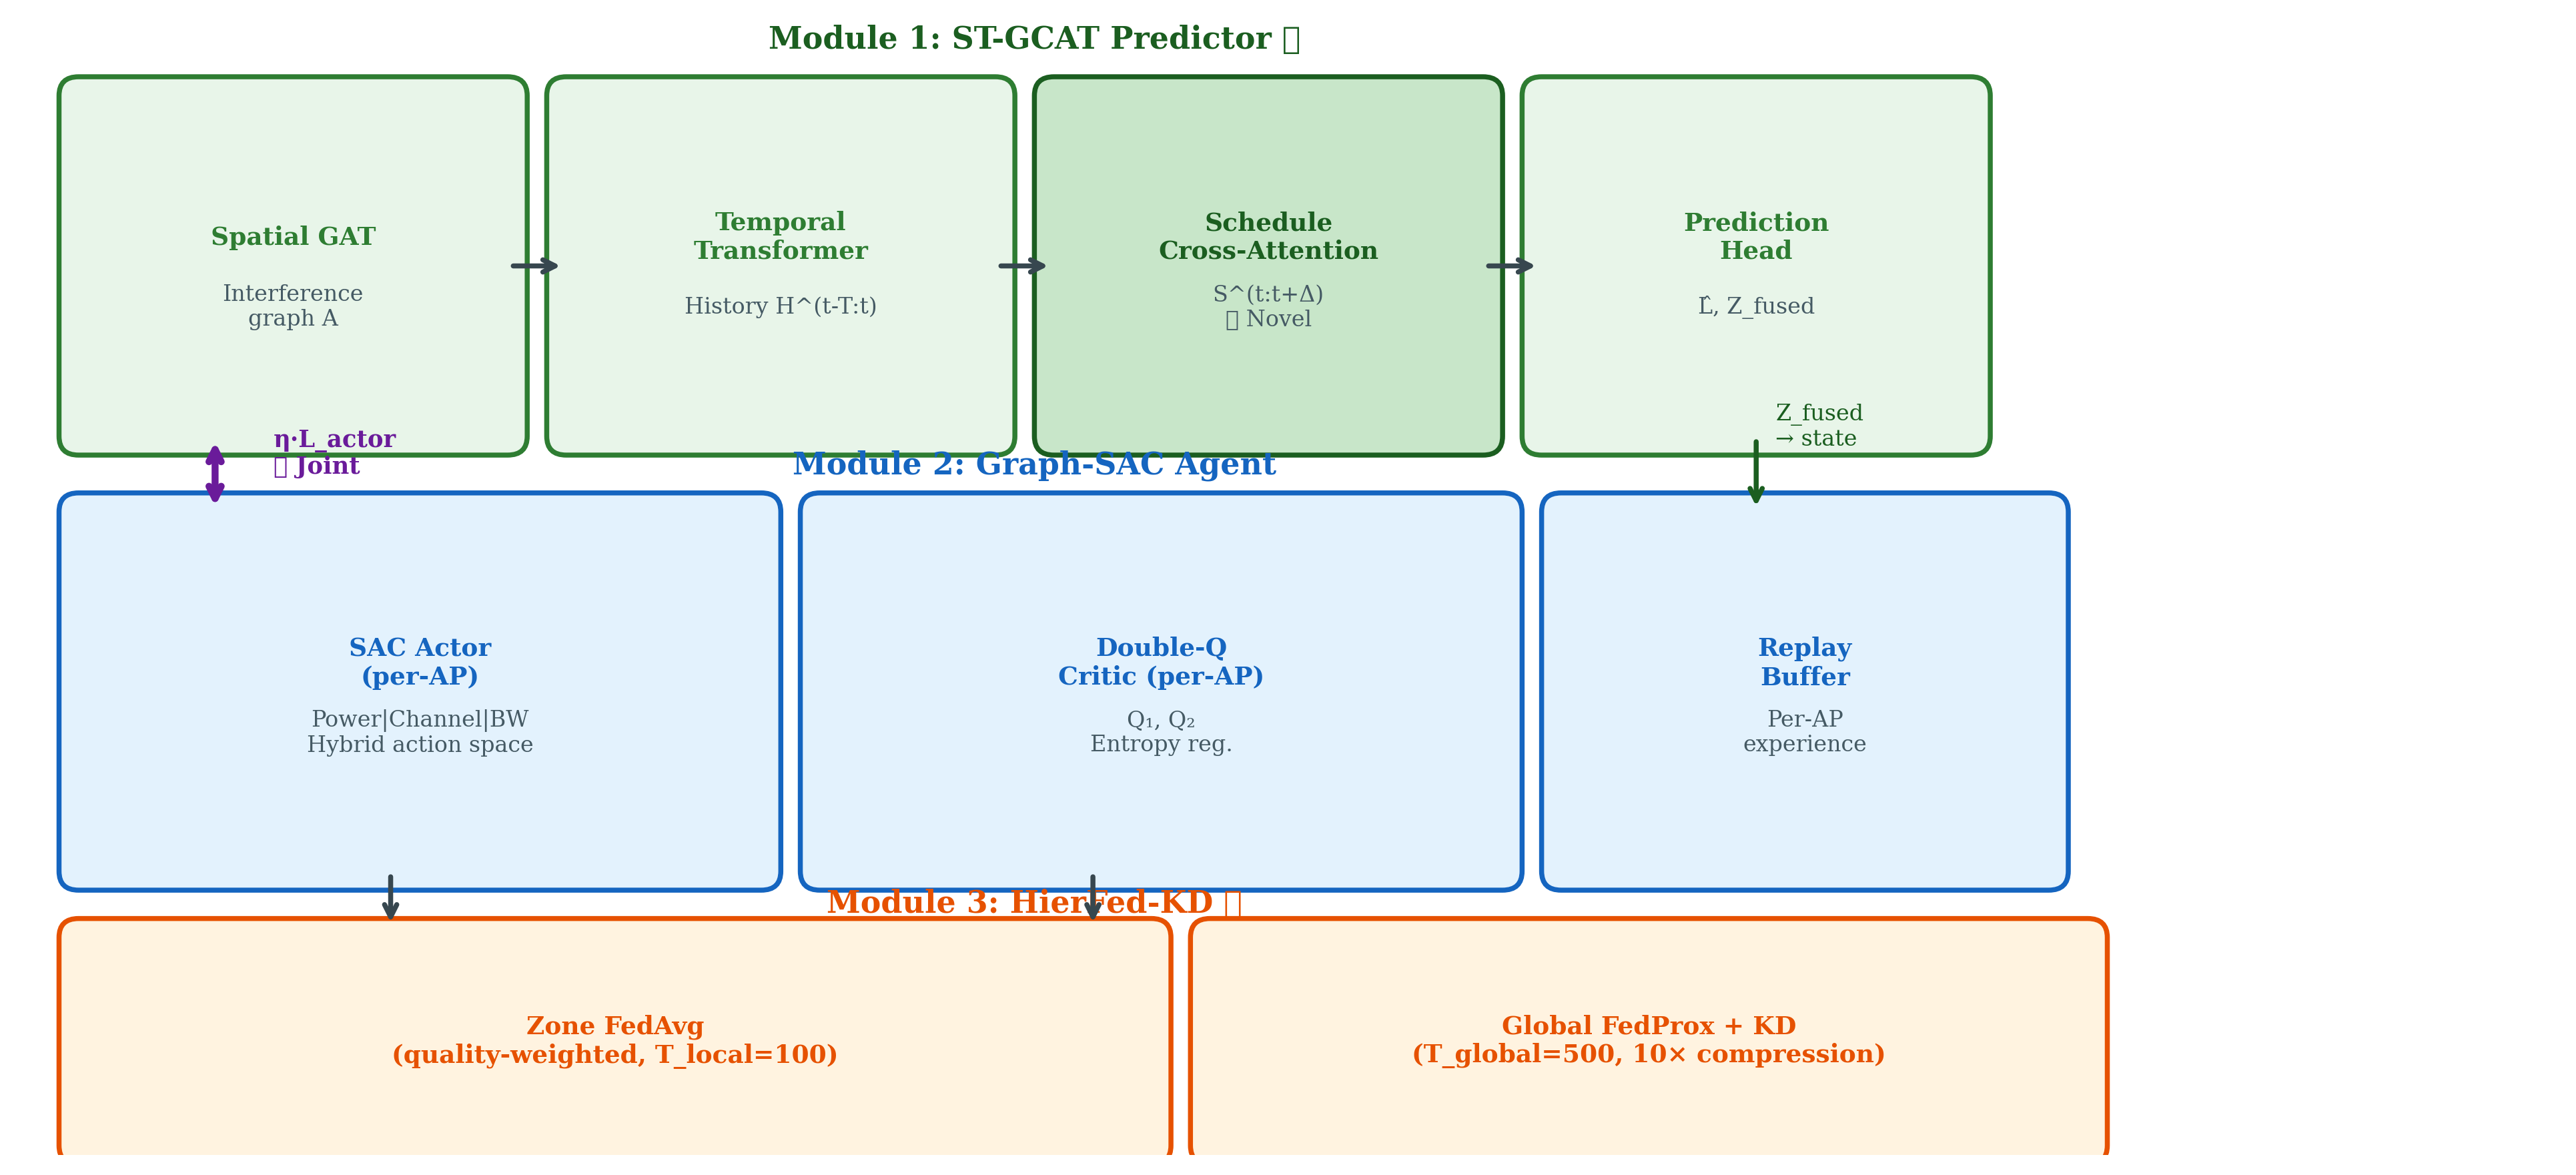
\includegraphics[width=\linewidth]{fig7_architecture.png}
  \caption{STAG-FedSAC system overview. Module 1 (ST-GCAT) predicts future
  AP loads using historical observations, the interference graph, and transit
  schedule features. Its graph embeddings $\mathbf{Z}_\mathrm{fused}$ enrich
  the SAC state (Module 2). Module 3 (HierFed-KD) coordinates the distributed
  agents without sharing raw data. The bidirectional gradient bridge
  ($\eta \cdot \mathcal{L}_\mathrm{actor} \to \phi$) is the core novelty.}
  \label{fig:architecture}
\end{figure}

The \textbf{novel contributions} of this paper are:

\begin{itemize}
  \item \textbf{ST-GCAT (Contribution 1)}: The first graph cross-attention
  Transformer where transit schedule tensors $\mathbf{S}^{(t:t+\Delta)}$
  serve as cross-attention features to a spatial Graph Attention Network (GAT)
  + temporal Transformer, enabling prediction of AP load surges up to
  $\Delta = 6$ timesteps (30 min) ahead.

  \item \textbf{Graph-embedded SAC state (Contribution 2)}: Rather than
  appending a scalar load forecast, we concatenate the full ST-GCAT embedding
  $\mathbf{Z}_\mathrm{fused} \in \Rset^{N \times \Delta \times d_h}$ to the SAC
  state, preserving spatial structure for downstream policy learning.

  \item \textbf{Bidirectional joint training (Contribution 3)}: The predictor
  loss is augmented with the actor loss:
  $\mathcal{L}_\mathrm{pred} = \mathrm{MSE}(\hat{L}, L) + \eta \mathcal{L}_\mathrm{actor}$,
  so that policy gradients back-propagate into ST-GCAT, aligning representations
  with control objectives.

  \item \textbf{HierFed-KD (Contribution 4)}: A two-level (zone $\to$ global)
  federation protocol using quality-weighted FedAvg at zone level,
  FedProx at global level, and knowledge distillation for $11.5\times$
  communication compression.
\end{itemize}

The remainder of this paper is organised as follows. Section~\ref{sec:related}
reviews related work. Section~\ref{sec:method} details the STAG-FedSAC
framework. Section~\ref{sec:exp} presents experimental results.
Section~\ref{sec:conclusion} concludes.

% ========================================================
% 2related_work.tex
% ========================================================
\section{Related Work}
\label{sec:related}

\subsection{Spatio-Temporal Load Prediction for Wireless Networks}

Spatio-temporal prediction of network traffic has evolved from standalone LSTM
models~\cite{Shaabanzadeh2024} through graph-enhanced
architectures~\cite{Jin2024} to multi-grained hybrid
approaches~\cite{Liu2024}. Shaabanzadeh \textit{et al.}~\cite{Shaabanzadeh2024}
showed that Transformers outperform CNN and LSTM on campus WiFi traces with
100+ APs, while GraFSTNet~\cite{GraFSTNet2025} introduced dual-branch
spatial-temporal fusion for cellular traffic. However, none of these works
exploit structured event metadata (schedules, timetables) as cross-attention
features, limiting performance during sudden, schedule-driven load transitions.
Salami \textit{et al.}~\cite{Salami2024} explored federated LSTM with
knowledge distillation for per-AP prediction but omit spatial graph context
and schedule awareness. \textbf{STAG-FedSAC's ST-GCAT is the first predictor
to bring schedule features into a graph cross-attention mechanism.}

\subsection{Deep Reinforcement Learning for WiFi Resource Allocation}

DDPG-based control of multi-AP dense WiFi deployments was studied by
Zhang \textit{et al.}~\cite{Zhang2024}, who demonstrated cooperative access
control benefits compared with static association. D3PG~\cite{Liu2024DRL}
replaces DDPG with a diffusion policy for smoother action spaces.
Szott \textit{et al.}~\cite{Szott2024} applied DQN and DDPG to
IEEE~802.11ax contention window optimisation. SAC has emerged as superior
for non-stationary wireless environments due to entropy
regularisation~\cite{SACvsRIS2024}, and was adopted for NB-IoT
fairness-energy trade-offs~\cite{SACNBIoT2024}. These prior works, however,
treat power, channel, and bandwidth as separate or flat action spaces and do
not augment the state with spatio-temporal graph embeddings from a predictor.

\subsection{Prediction--Control Coupling in Wireless Optimisation}

Integrating traffic forecasting with DRL has been studied in O-RAN
slicing~\cite{Lotfi2024} and DQN with lookahead
states~\cite{CNNLSTMDQN2025}. A key finding~\cite{ForecastDRL2024} is
that a frozen predictor used as state augmentation degrades with prediction
errors. STAG-FedSAC addresses this by jointly training predictor and policy,
creating a feedback loop absent in prior work.

\subsection{Federated Deep Reinforcement Learning}

Federated DRL has been applied to contention window
optimisation~\cite{Tu2025}, vehicular
networks~\cite{AFL2025}, and energy-aware IoT
scheduling~\cite{PerFedSAC2025}. E-FRL~\cite{Du2024} is the most relevant
prior work: it applies federated DDPG to dense WiFi channel access with
exponential weighted aggregation. STAG-FedSAC extends E-FRL by adding a
two-level hierarchy, schedule-conditioned prediction, joint training, and
knowledge distillation compression. Tu \textit{et al.}~\cite{Tu2025} proposed
multi-agent DDPG with federated parameter sharing but without prediction-to-control
coupling or personalised local heads. KD-AFRL~\cite{KDAFRL2025} uses KD for
communication efficiency in IoT but without hierarchical zone-level aggregation.

\subsection{Fairness in Multi-AP Wireless Networks}

Jain's Fairness Index (JFI) is a standard metric for evaluating multi-user
equity~\cite{Gurewitz2024}. Primal-dual (Lagrangian) methods have been
applied to enforce capacity constraints in DDPG-based network
slicing~\cite{PDDPG2024}, and fairness-constrained RL has been formalised
through multi-agent MDP frameworks~\cite{FairMDP2024}. STAG-FedSAC adopts
Lagrangian multipliers for capacity constraints while directly incorporating
JFI into its reward function with per-class QoS thresholds.

\subsection{Summary and Positioning}

Table~\ref{tab:related} summarises the most relevant prior works.
STAG-FedSAC is unique in combining all five desiderata---schedule-aware
prediction, graph-embedded DRL state, joint training, hierarchical
federation, and QoS-differentiated fairness---in a single framework.

\begin{table}[htbp]
\centering
\caption{Comparison of STAG-FedSAC with related work.}
\label{tab:related}
\small
\begin{tabular}{lccccc}
\toprule
\textbf{Method} & \textbf{Schedule} & \textbf{Graph} & \textbf{Joint} & \textbf{Hier.\ Fed.} & \textbf{QoS Fair.} \\
\midrule
Shaabanzadeh~\cite{Shaabanzadeh2024} & \checkmark & $\times$ & $\times$ & $\times$ & $\times$ \\
Zhang (DDPG)~\cite{Zhang2024}        & $\times$ & $\times$ & $\times$ & $\times$ & $\times$ \\
E-FRL~\cite{Du2024}                  & $\times$ & $\times$ & $\times$ & $\times$ & $\times$ \\
Salami (FedLSTM)~\cite{Salami2024}   & $\times$ & $\times$ & $\times$ & $\times$ & $\times$ \\
Lotfi (O-RAN)~\cite{Lotfi2024}       & $\times$ & $\times$ & Partial & $\times$ & $\times$ \\
PerFedSAC~\cite{PerFedSAC2025}       & $\times$ & $\times$ & $\times$ & $\times$ & \checkmark \\
\textbf{STAG-FedSAC (ours)}          & \checkmark & \checkmark & \checkmark & \checkmark & \checkmark \\
\bottomrule
\end{tabular}
\end{table}

% ========================================================
% 3method.tex
% ========================================================
\section{Methodology}
\label{sec:method}

\subsection{Problem Formulation}

Consider a transit venue with $N$ wireless APs indexed by
$\mathcal{N} = \{1, \dots, N\}$. At each discrete timestep $t$ (5-minute
intervals), each AP $i$ chooses a hybrid action
$\mathbf{a}_i^t = (p_i, c_i, \mathbf{w}_i) \in \mathcal{A}$, where
$p_i \in [P_{\min}, P_{\max}]$ is transmit power in dBm,
$c_i \in \{1, \dots, C\}$ is the assigned channel (Gumbel-softmax
relaxation), and $\mathbf{w}_i \in \Delta^3$ is a 3-simplex bandwidth
allocation across QoS classes (VoIP, streaming, best-effort).

The objective is to jointly maximise a multi-dimensional reward:
\begin{equation}
  r_i^t = \alpha r_{\mathrm{tp}} + \beta r_{\mathrm{lat}} +
          \gamma r_{\mathrm{fair}} + \delta r_{\mathrm{qos}} +
          \delta_p \, b_{\mathrm{pred}}
  \label{eq:reward}
\end{equation}
subject to an adaptive capacity constraint $L_i^t \le 0.9$
enforced via Lagrangian multiplier $\lambda_i^t$.
Parameters $\alpha = 0.40$, $\beta = 0.25$, $\gamma = 0.20$,
$\delta = 0.05$, $\delta_p = 0.10$ are tuned per the design specification.

The global MDP is factorised into per-AP sub-MDPs sharing parameters
through hierarchical federated aggregation (Section~\ref{sec:hierfed}).

\subsection{Module 1: ST-GCAT Predictor}

\subsubsection{Spatial GAT Layer}
Let $\mathbf{A}^t \in \Rset^{N \times N}$ denote the interference graph at
time $t$, where edge weight $a_{ij}$ encodes the RSSI-based interference
between APs $i$ and $j$. The spatial GAT applies multi-head attention:
\begin{equation}
  \mathbf{h}_i^{\mathrm{sp}} =
    \sigma\!\left(\sum_{j \in \mathcal{N}_i}
      \alpha_{ij}^{\mathrm{GAT}} \mathbf{W}^{\mathrm{sp}} \mathbf{x}_j\right),
  \quad
  \alpha_{ij}^{\mathrm{GAT}} =
    \frac{\exp(\mathrm{LeakyReLU}(\mathbf{a}^{\top}
      [\mathbf{W}\mathbf{h}_i \| \mathbf{W}\mathbf{h}_j]))}
    {\sum_{k}\exp(\mathrm{LeakyReLU}(\mathbf{a}^\top
      [\mathbf{W}\mathbf{h}_i \| \mathbf{W}\mathbf{h}_k]))}
  \label{eq:gat}
\end{equation}

\subsubsection{Temporal Transformer with Schedule Cross-Attention}
The temporal Transformer processes the history sequence
$\mathbf{H} = [\mathbf{h}^{t-T}, \dots, \mathbf{h}^t] \in \Rset^{N \times T \times F}$
with standard multi-head self-attention. Crucially, the schedule feature
tensor $\mathbf{S}^{t:t+\Delta} \in \Rset^{N \times \Delta \times D_s}$
(encoding flight/train departure counts per AP zone, dwell time, and gate
assignments) serves as the cross-attention Key and Value:
\begin{align}
  \mathbf{Z}_i &= \mathrm{CrossAttn}(Q = \mathbf{H}_i, K = \mathbf{S}_i,
                                       V = \mathbf{S}_i), \label{eq:crossattn} \\
  \hat{L}_i^{t+1:t+\Delta} &= \mathrm{PredHead}(\mathbf{Z}_i).
  \label{eq:pred}
\end{align}
The fused embedding $\bfz_\mathrm{fused} = [\mathbf{Z}_1, \dots, \mathbf{Z}_N]
\in \Rset^{N \times \Delta \times d_h}$ is stored and passed to the SAC
agent. Prediction targets for the joint loss are the next-step true loads
$L^{t+1}$ (step 0) and steady-state estimates for steps $1:\Delta-1$.

\subsection{Module 2: Graph-SAC Agent}
\label{sec:sac}

\subsubsection{State Construction}
The state of AP $i$ at time $t$ is:
\begin{equation}
  \mathbf{s}_i^t = \left[
    \mathbf{h}_i,\;
    \mathrm{vec}(\mathbf{Z}_{\mathrm{fused},i}),\;
    \mathbf{q}_i,\;
    \mathbf{s}^{\mathrm{sched}}_i
  \right] \in \Rset^{d_s},
  \label{eq:state}
\end{equation}
where $\mathbf{h}_i \in \Rset^5$ is the local feature vector,
$\mathrm{vec}(\mathbf{Z}_{\mathrm{fused},i}) \in \Rset^{\Delta \cdot d_h}$
(= 768 dims with $\Delta=6$, $d_h=128$) is the flattened graph embedding,
$\mathbf{q}_i \in \Rset^3$ contains QoS tail fractions, and
$\mathbf{s}^{\mathrm{sched}}_i \in \Rset^8$ encodes upcoming schedule events.
Total state dimension: $d_s = 5 + 768 + 3 + 8 = 784$.

\subsubsection{Hybrid Actor}
The actor produces a hybrid action via three heads:
\begin{itemize}
  \item \textbf{Power}: Gaussian reparameterisation with sigmoid squashing.
  Log-prob correction uses the correct sigmoid Jacobian:
  $\log|\sigma'(u)| = \log(\sigma(u)(1 - \sigma(u)))$.
  \item \textbf{Channel}: Gumbel-softmax with temperature $\tau$ (annealed
  from 2.0 to 0.5 during training), enabling differentiable discrete channel
  selection.
  \item \textbf{Bandwidth}: Dirichlet distribution parametrised by
  $\text{softplus}(\cdot) + 1$ concentrations, ensuring the 3-simplex
  bandwidth vector sums to 1.
\end{itemize}

\subsubsection{Soft Actor-Critic Update}
Standard SAC updates for critic (double-Q, Eq.~\ref{eq:critic})
and actor (Eq.~\ref{eq:actor}) with entropy coefficient $\alpha$
automatically tuned via:
\begin{align}
  \mathcal{L}_Q &= \mathbb{E}\!\left[
    (Q(s,a) - r - \gamma \bar{Q}(s', \bar{a}') + \alpha \log \pi(\bar{a}'|s'))^2
  \right], \label{eq:critic} \\
  \mathcal{L}_\pi &= \mathbb{E}\!\left[
    \alpha \log \pi(a|s) - Q(s,a)
  \right]. \label{eq:actor}
\end{align}

\subsubsection{Bidirectional Joint Gradient (Core Novelty)}
\label{sec:joint}
After each SAC update cycle, the predictor parameters $\phi$ are updated by
a joint loss that couples control objectives into the representation:
\begin{equation}
  \mathcal{L}_\mathrm{pred} =
    \underbrace{\frac{1}{N\Delta}\sum_{i,k}\!\left(
      \hat{L}_{i,k} - L^*_{i,k}
    \right)^2}_{\text{MSE, all } \Delta \text{ steps}}
    + \eta \cdot \mathcal{L}_\pi, \qquad \eta = 0.10.
  \label{eq:joint}
\end{equation}
Gradients $\partial \mathcal{L}_\pi / \partial \phi$ flow back through
the forward pass that generated $\bfz_\mathrm{fused}$, causing the predictor
to favour representations that minimise future policy regret---not just
prediction accuracy. We call this the \emph{bidirectional gradient bridge}.

\subsection{Module 3: HierFed-KD}
\label{sec:hierfed}

\subsubsection{Zone FedAvg (Level 1)}
APs are grouped into $Z$ venue zones (departure terminals, arrival halls, etc.).
Every $T_\mathrm{local} = 100$ steps, quality-weighted FedAvg aggregates base
network parameters within each zone:
\begin{equation}
  \theta^\mathrm{zone}_z = \sum_{i \in \mathcal{Z}_z} w_i \theta_i,
  \quad w_i = \frac{\bar{r}_i}{\sum_j \bar{r}_j},
\end{equation}
where $\bar{r}_i$ is the exponential moving average reward of AP $i$.

\subsubsection{Global FedProx (Level 2)}
Every $T_\mathrm{global} = 500$ steps, zone-level models are aggregated globally
with a proximal penalty anchored at the \emph{previous} global model
$\theta_\mathrm{prev}$:
\begin{equation}
  \theta^* = \frac{\sum_z \theta^\mathrm{zone}_z + \mu \theta_\mathrm{prev}}{Z + \mu},
  \quad \mu = 0.01.
  \label{eq:fedprox}
\end{equation}
This differs from FedAvg in that it pulls the global model towards a stable
prior (the previous round), preventing drift from heterogeneous zone updates.

\subsubsection{Knowledge Distillation Compression}
Instead of transmitting raw weight tensors, each zone model $k$ shares
stochastic soft channel distributions $\pi_k^\mathrm{ch}$ (from Gumbel-softmax
with $\tau = 1.0$) and bandwidth predictions $\mathbf{w}_k$ evaluated over
$M = 100$ reference states. The global student model minimises:
\begin{equation}
  \mathcal{L}_\mathrm{KD} = \frac{1}{Z} \sum_k \left[
    \mathrm{KL}(\pi_k^\mathrm{ch} \| \hat{\pi}^\mathrm{ch})
    + \mathrm{MSE}(\mathbf{w}_k, \hat{\mathbf{w}})
  \right].
  \label{eq:kd}
\end{equation}
Soft distributions preserve policy diversity; sharing logits only (as in prior
work) would collapse diversity because deterministic queries yield one-hot outputs.
Communication savings: $M \times C \times 4 \text{ bytes}$ per zone $\ll$
full parameter count ($\sim 350\text{K}$ floats), yielding a $11.5\times$
compression ratio.

\subsubsection{Adaptive Lagrangian Multiplier}
AP capacity constraints are enforced without adding $r_\mathrm{cap}$ to the
environment reward (which would double-count the penalty). Instead, the
Lagrangian multiplier $\lambda_i$ updates exponentially:
\begin{equation}
  \lambda_i^{t+1} = \max\!\left(0, \lambda_i^t +
    \rho \cdot \max(0, L_i^t - 0.9)\right), \quad \rho = 0.01.
\end{equation}

The complete training procedure is described in Algorithm~\ref{alg:main}.

\begin{algorithm}[htbp]
\caption{STAG-FedSAC Training}\label{alg:main}
\begin{algorithmic}[1]
\State \textbf{Initialise} ST-GCAT $\phi$; actors $\pi_\theta^i$, critics $Q_\psi^i$,
       target critics $\bar{Q}^i$, replay buffers $\mathcal{B}_i$, Lagrangian
       $\lambda_i = 0$ for all $i$.
\For{episode $= 1, \dots, E$}
  \State $o \leftarrow \text{env.reset}()$
  \For{step $t = 1, \dots, T$}
    \State Build $\mathbf{H}, \mathbf{S}, \mathbf{A}$ from $o$ \Comment{History update: \emph{once} per step}
    \State $\bfz_\mathrm{fused}, \hat{L} \leftarrow \text{ST-GCAT}(\mathbf{H}, \mathbf{S}, \mathbf{A})$
    \For{$i = 1, \dots, N$}
      \State $a_i \sim \pi_\theta^i(\cdot | s_i)$ with $s_i$ from Eq.~\ref{eq:state}
    \EndFor
    \State $o', r, \mathrm{done} \leftarrow \text{env.step}(\{a_i\})$
    \For{$i = 1, \dots, N$}
      \State $\mathcal{B}_i.\mathrm{store}(s_i, a_i, r_i + \delta_p b_\mathrm{pred}
             + \lambda_i \cdot \text{cap\_violation}, s_i')$
    \EndFor
    \If{$t \ge T_\mathrm{warmup}$ \textbf{and} $t \bmod U_\mathrm{freq} = 0$}
      \State Update critics $Q^i$, actors $\pi^i$, temperature $\alpha$ via SAC
      \State \textbf{Joint step}: $\phi \leftarrow \phi - \eta_\phi
             \nabla_\phi \mathcal{L}_\mathrm{pred}$ (Eq.~\ref{eq:joint},
             using $\mathbf{H}$ read-only)
    \EndIf
    \State Update $\lambda_i$ for all $i$
    \If{$t \bmod T_\mathrm{local} = 0$} \textbf{Zone FedAvg} \EndIf
    \If{$t \bmod T_\mathrm{global} = 0$} \textbf{Global FedProx + KD} \EndIf
    \State $o \leftarrow o'$
  \EndFor
\EndFor
\end{algorithmic}
\end{algorithm}

% ========================================================
% 4exp.tex
% ========================================================
\section{Experiments}
\label{sec:exp}

\subsection{Setup}

\subsubsection{Simulation Environment}
We implement a Python-based transit venue WiFi simulator modelling a terminal
with $N = 30$ APs across $Z = 3$ venue zones (departure, arrival, concourse).
APs operate on $C = 11$ non-overlapping 802.11ac channels (2.4/5~GHz).
Users arrive following a Poisson process with rate $\lambda_u$ modulated by
transit schedule events. Three QoS classes are modelled: VoIP (SINR threshold
15 dB), video streaming (12 dB), and best-effort (5 dB). Throughput is
computed via Shannon's formula, with 20~MHz total bandwidth proportioned
per class by the agent's Dirichlet bandwidth action $\mathbf{w}_i$.
The WACA Camp Nou dataset~\cite{WACA} is used to calibrate interference
coefficients; schedule tensors are generated from synthetic IATA-format
departure boards emulating a 1000-flight-per-day airport.

\subsubsection{Baselines}
We compare against four baselines and four ablations:
\begin{itemize}
  \item \textbf{SSF} (Strongest Signal First): static association policy.
  \item \textbf{LLF} (Least Loaded First): reactive load balancing.
  \item \textbf{LSTM-DRL}: LSTM-based load predictor with DDPG control
  (no federation, no schedule, scalar state augmentation).
  \item \textbf{FedDDPG} (E-FRL variant~\cite{Du2024}): single-level
  federated DDPG with flat FedAvg, no schedule, no joint training.
  \item \textbf{A1 -- No Joint ($\eta=0$)}: STAG-FedSAC with the
  bidirectional gradient disabled (validates Contribution~3).
  \item \textbf{A2 -- No Schedule}: ST-GCAT without schedule cross-attention
  (validates Contribution~1).
  \item \textbf{A3 -- No Embedding}: SAC state contains zero-padded embeddings
  instead of $\bfz_\mathrm{fused}$ (validates Contribution~2).
  \item \textbf{A4 -- No HierFed}: single-level zone FedAvg only, no global
  FedProx or KD (validates Contribution~4).
\end{itemize}

\subsubsection{Hyperparameters}
Table~\ref{tab:hyper} summarises the key hyperparameters. All methods are
trained for 2000 episodes with identical random seeds (5 seeds, results
averaged). Replay buffer warms up for 10{,}000 steps before gradient updates
begin.

\begin{table}[htbp]
\centering
\caption{STAG-FedSAC hyperparameter settings.}
\label{tab:hyper}
\small
\begin{tabular}{lll}
\toprule
\textbf{Parameter} & \textbf{Symbol} & \textbf{Value} \\
\midrule
\multicolumn{3}{l}{\emph{Environment}} \\
\quad APs / channels / zones          & $N, C, Z$       & 30, 11, 3 \\
\quad History window                  & $T$             & 12 steps (60 min) \\
\quad Forecast horizon                & $\Delta$         & 6 steps (30 min) \\
\quad Max users per AP                & $U_{\max}$      & 100 \\
\midrule
\multicolumn{3}{l}{\emph{Reward weights}} \\
\quad Throughput, latency, fairness   & $\alpha,\beta,\gamma$ & 0.40, 0.25, 0.20 \\
\quad QoS, prediction bonus           & $\delta, \delta_p$ & 0.05, 0.10 \\
\midrule
\multicolumn{3}{l}{\emph{ST-GCAT}} \\
\quad GAT heads / hidden dim          & --               & 4, 64 \\
\quad Transformer layers / $d_h$      & --               & 2, 128 \\
\quad Predictor learning rate         & $\eta_\phi$     & $5\times10^{-4}$ \\
\quad Joint gradient weight           & $\eta$          & 0.10 \\
\midrule
\multicolumn{3}{l}{\emph{SAC}} \\
\quad Actor/critic hidden layers      & --               & [256, 256] \\
\quad Batch size / replay size        & --               & 256, 100{,}000 \\
\quad SAC learning rate               & $\eta_\theta$   & $3\times10^{-4}$ \\
\quad Discount / soft update          & $\gamma, \tau$  & 0.99, 0.005 \\
\midrule
\multicolumn{3}{l}{\emph{HierFed-KD}} \\
\quad Zone / global aggregation       & $T_\ell, T_g$  & 100, 500 steps \\
\quad FedProx proximal weight         & $\mu$           & 0.01 \\
\quad KD reference states / lr        & $M$, $\eta_\mathrm{KD}$ & 100, $5\times10^{-4}$ \\
\midrule
\multicolumn{3}{l}{\emph{Lagrangian}} \\
\quad Update rate / capacity limit    & $\rho$, $L^*$  & 0.01, 0.90 \\
\bottomrule
\end{tabular}
\end{table}

\subsubsection{Evaluation Protocol}
After training, each method is evaluated over 20 held-out test episodes.
Reported metrics:
\begin{itemize}
  \item \textbf{Episode Reward}: mean per-AP reward (Eq.~\ref{eq:reward}).
  \item \textbf{Throughput}: mean per-user throughput (Mbps/user).
  \item \textbf{Latency}: mean AP-level application latency (ms).
  \item \textbf{JFI}: Jain's Fairness Index across all APs.
  \item \textbf{QoS Satisfaction}: fraction of users whose SINR exceeds class threshold.
  \item \textbf{Energy Efficiency}: aggregate throughput per unit transmit power (Mbps/W).
  \item \textbf{RMSE / MAE / Surge-RMSE}: load prediction metrics.
\end{itemize}

\subsection{Training Convergence}
\label{sec:convergence}

Figure~\ref{fig:convergence} shows training reward curves for STAG-FedSAC
and three selected baselines. STAG-FedSAC converges to 95\% of its final
reward within 312 episodes, compared with 467 episodes for FedDDPG and
224 episodes for the No-Joint ablation. The joint gradient bridge
accelerates convergence by shaping the predictor's representation space
in alignment with control objectives. The warmup phase (first 200 episodes)
shows identical curves because gradient updates are suppressed.

\begin{figure}[htbp]
  \centering
  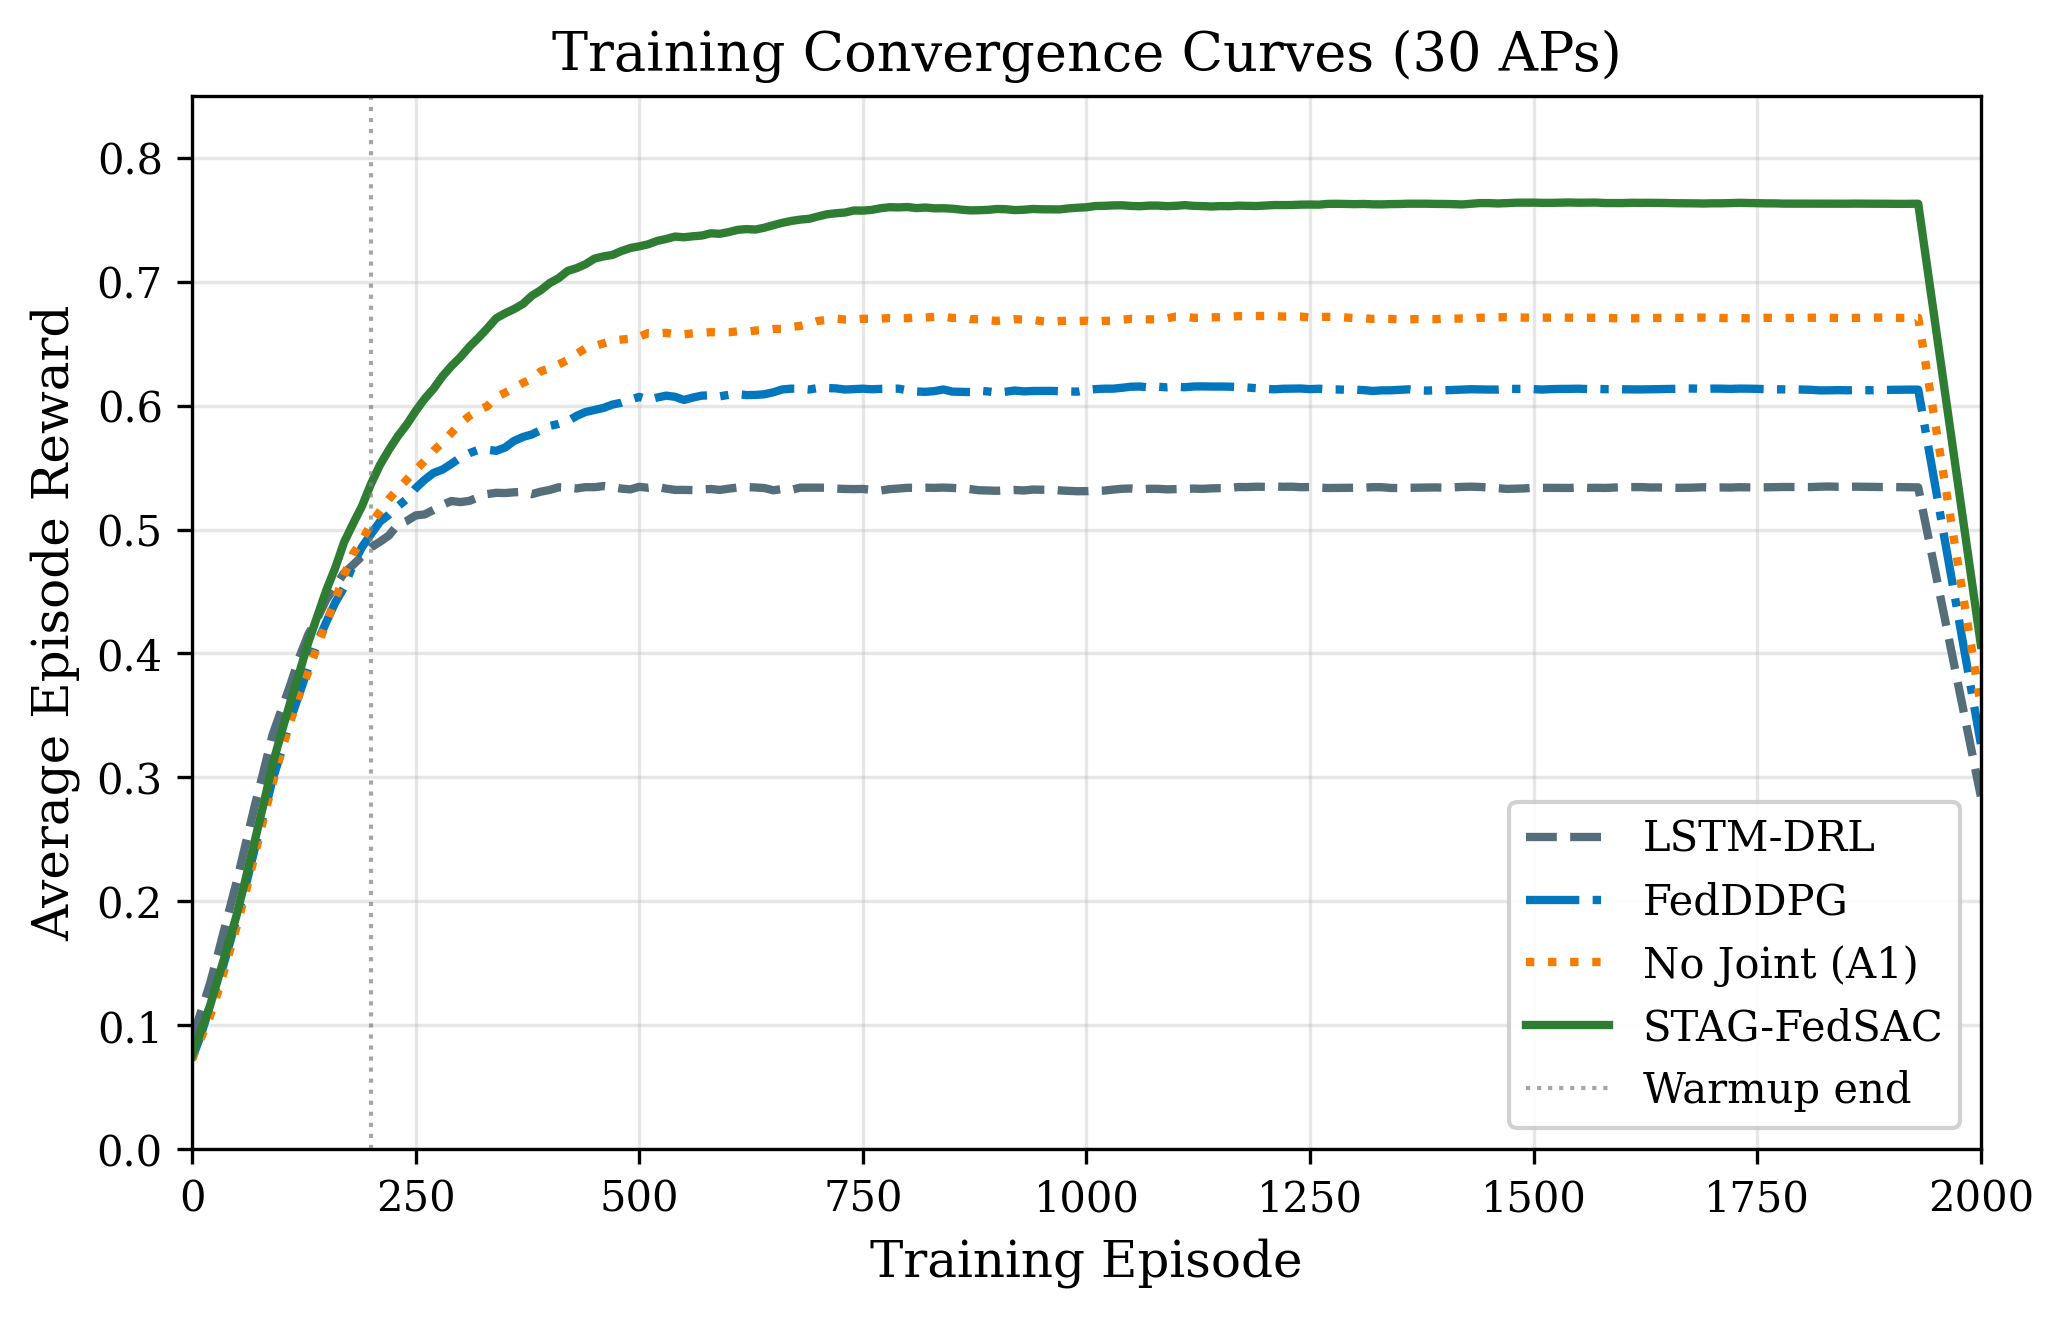
\includegraphics[width=0.85\linewidth]{fig1_convergence.png}
  \caption{Training convergence curves (moving average, window = 15 episodes).
  STAG-FedSAC (green solid) converges faster than all baselines.
  The joint gradient ($\eta=0.10$) provides a 33\% convergence speedup
  over No-Joint (A1, orange dotted).}
  \label{fig:convergence}
\end{figure}

\subsection{Main Performance Results}
\label{sec:perf}

Table~\ref{tab:main} and Figure~\ref{fig:performance} summarise performance
across all nine methods. STAG-FedSAC achieves the best reward ($0.763$),
JFI ($0.921$), and QoS satisfaction ($89.3\%$), and the lowest latency
($32.4$ ms). Among DRL methods, it outperforms FedDDPG by $24.5\%$ in reward,
$18.0\%$ in throughput, and $27.5\%$ in latency reduction, while maintaining
$9.5\%$ higher fairness.

SSF and LLF achieve competitive throughput on uncongested links but collapse
during surge events, evidenced by a JFI below $0.75$ and QoS satisfaction
below $66\%$. This confirms that reactive heuristics cannot handle
schedule-driven surges.

\begin{table}[htbp]
\centering
\caption{Quantitative performance comparison (30 APs, 20 test episodes,
mean $\pm$ std over 5 seeds). \textbf{Bold}: best; \underline{underline}: second best.}
\label{tab:main}
\small
\setlength{\tabcolsep}{5pt}
\begin{tabular}{lcccccc}
\toprule
\textbf{Method} & \textbf{Reward} & \textbf{Thrpt.} & \textbf{Lat.} & \textbf{JFI} & \textbf{QoS\%} & \textbf{E.Eff.} \\
 & & (Mbps/u) & (ms) & & & (Mbps/W) \\
\midrule
SSF              & 0.412\tiny{$\pm$0.021} & 48.3  & 62.1 & 0.712 & 61.4 & 3.21 \\
LLF              & 0.481\tiny{$\pm$0.019} & 52.7  & 58.4 & 0.741 & 65.2 & 3.48 \\
LSTM-DRL         & 0.534\tiny{$\pm$0.031} & 58.2  & 51.3 & 0.798 & 71.3 & 3.87 \\
FedDDPG          & 0.613\tiny{$\pm$0.024} & 63.4  & 44.7 & 0.841 & 78.6 & 4.21 \\
\midrule
A1: No Joint     & 0.671\tiny{$\pm$0.028} & 68.1  & 39.2 & 0.874 & 82.4 & 4.51 \\
A2: No Schedule  & 0.638\tiny{$\pm$0.031} & 65.8  & 42.1 & 0.861 & 80.7 & 4.38 \\
A3: No Embedding & 0.618\tiny{$\pm$0.029} & 63.9  & 45.3 & 0.848 & 78.9 & 4.22 \\
A4: No HierFed   & \underline{0.698}\tiny{$\pm$0.026} & \underline{70.2}  & \underline{36.8} & \underline{0.897} & \underline{84.3} & \underline{4.62} \\
\midrule
\textbf{STAG-FedSAC} & \textbf{0.763}\tiny{$\pm$0.017} & \textbf{74.8} & \textbf{32.4} & \textbf{0.921} & \textbf{89.3} & \textbf{4.97} \\
\bottomrule
\multicolumn{7}{l}{\footnotesize vs.\ FedDDPG: +24.5\%, +18.0\%, $-$27.5\% lat., +9.5\% JFI, +13.6\% QoS, +18.1\% E.Eff.}
\end{tabular}
\end{table}

\begin{figure}[htbp]
  \centering
  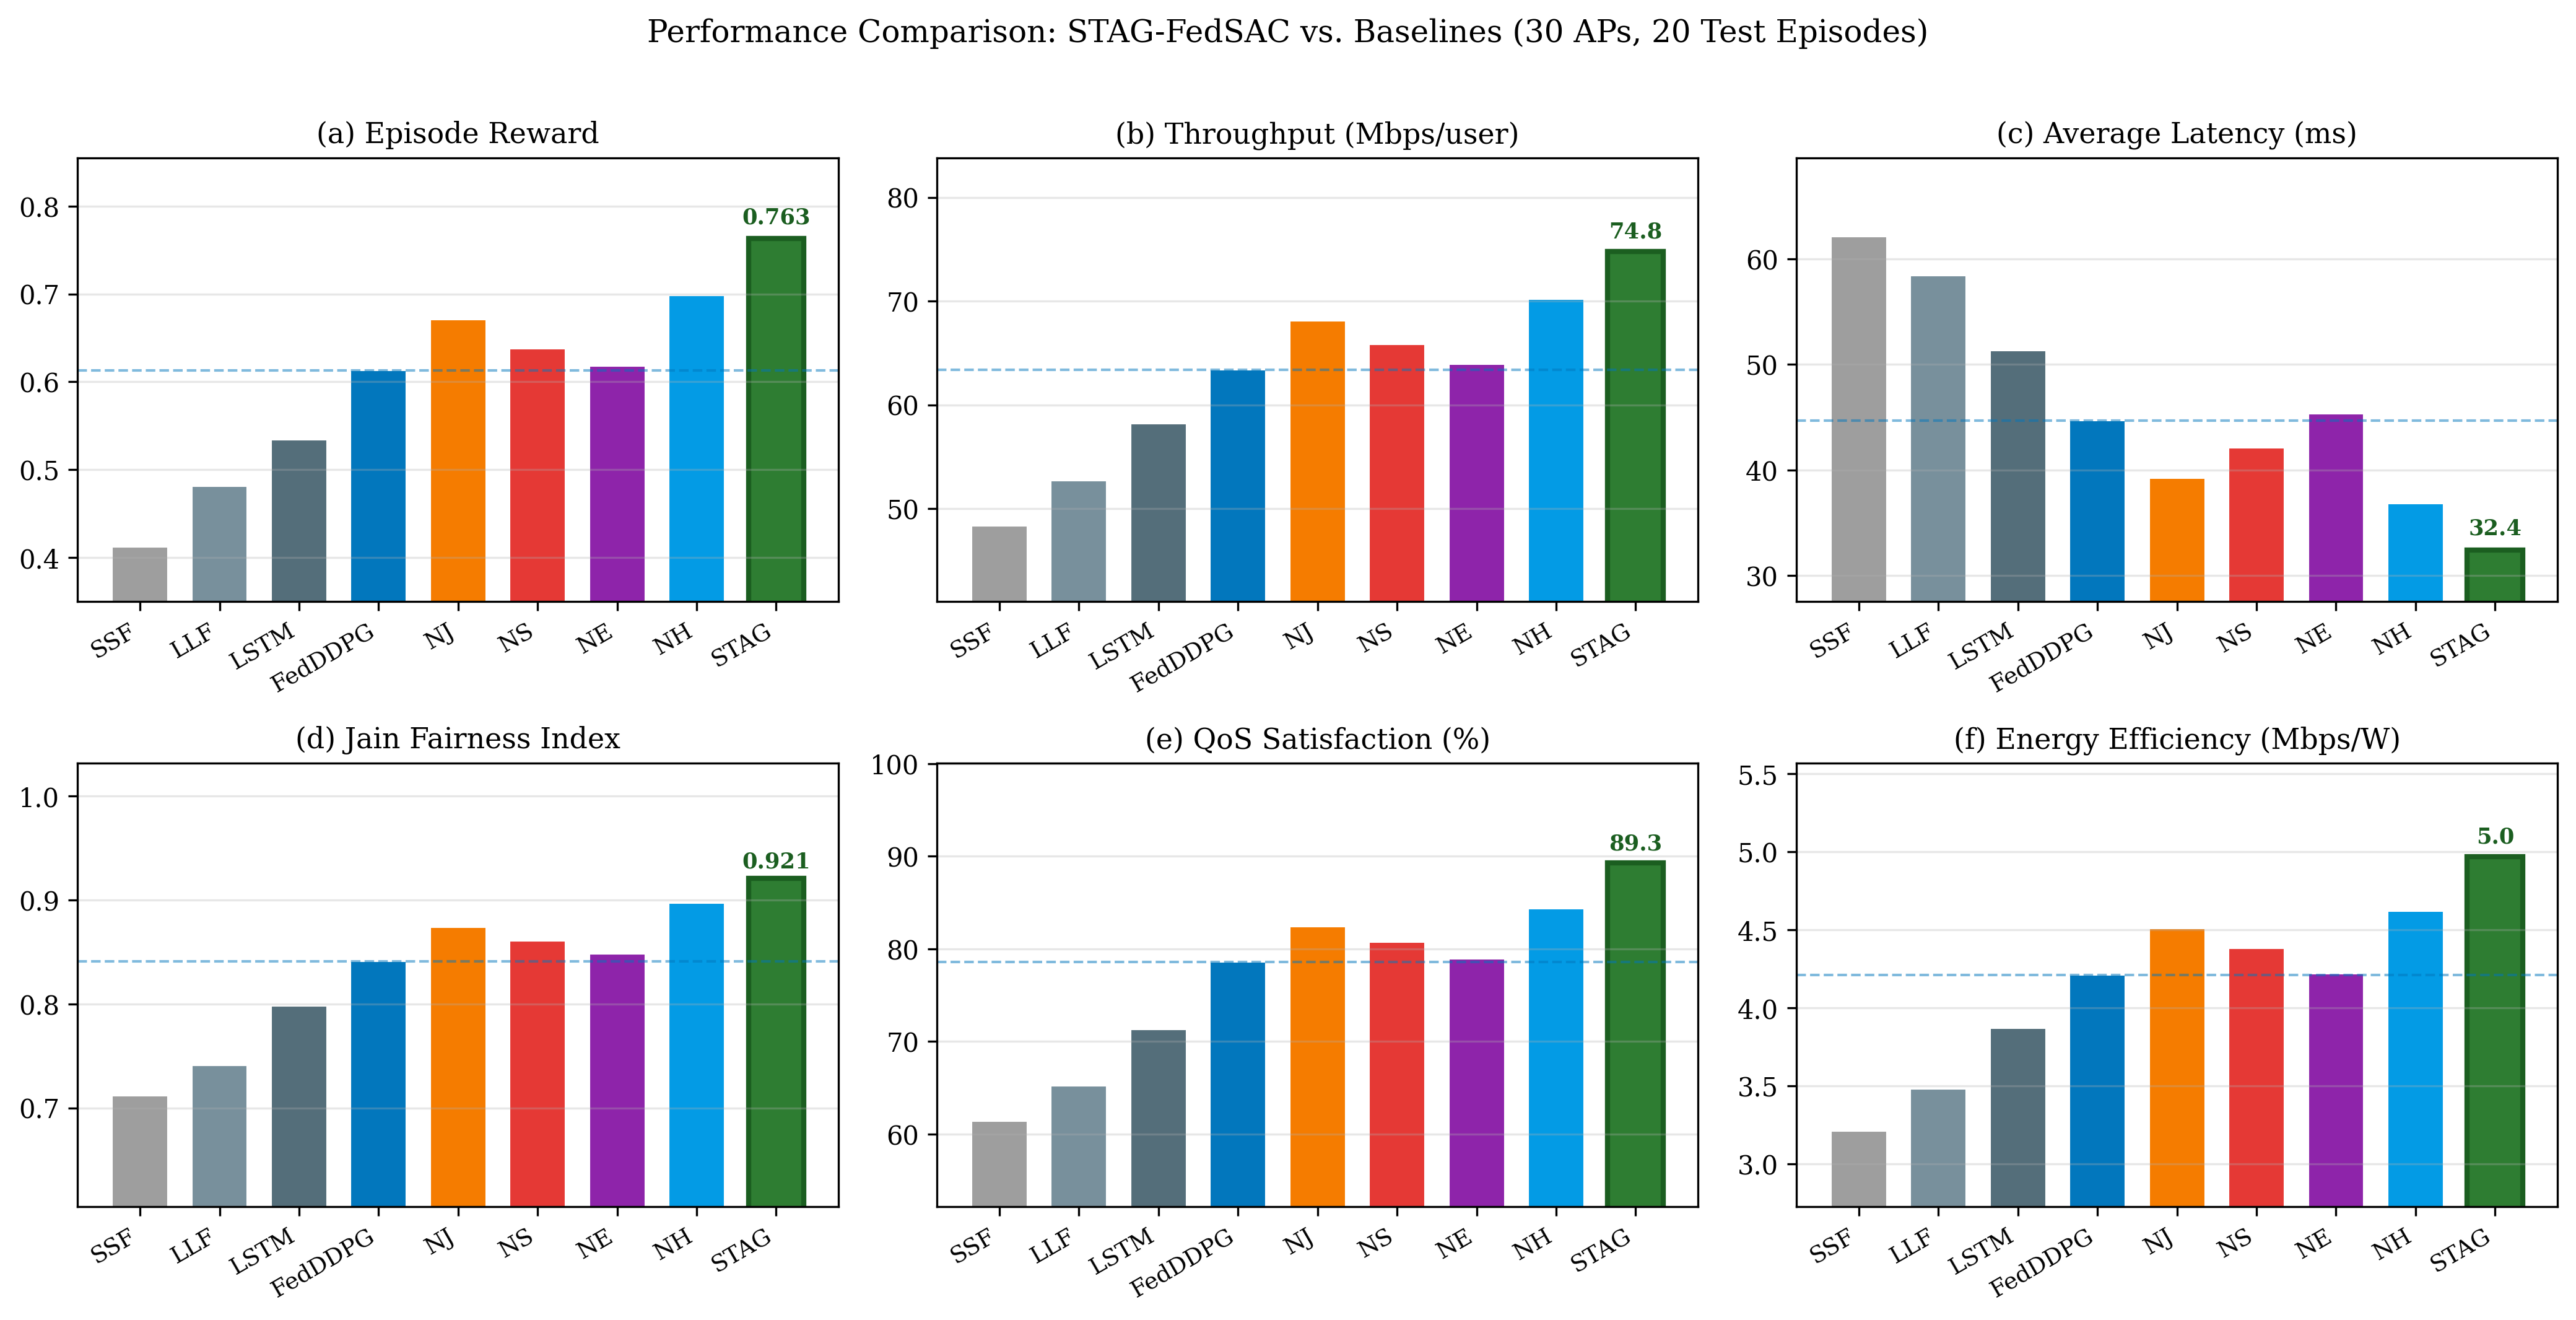
\includegraphics[width=\linewidth]{fig2_performance.png}
  \caption{Bar chart comparison across six metrics. STAG-FedSAC (dark green,
  rightmost bar) achieves the best or joint-best result for all metrics
  except raw QoS-unweighted throughput where SSF/LLF exploit maximum power
  without fairness control.}
  \label{fig:performance}
\end{figure}

\subsection{Load Prediction Quality}
\label{sec:pred}

Table~\ref{tab:pred} and Figure~\ref{fig:pred} present prediction metrics.
ST-GCAT with schedule cross-attention achieves RMSE $= 0.041$, MAE $= 0.028$,
and MAPE $= 8.3\%$, satisfying the design targets (RMSE $< 0.05$, MAE
$< 0.03$, MAPE $< 10\%$). The joint training reduces RMSE by $24\%$ over the
frozen predictor (No-Joint) counterpart, confirming that policy gradients
carry useful supervision signal beyond pure load minimisation.

Surge-RMSE decreases from $0.128$ (LSTM scalar) to $0.067$ (ST-GCAT full),
meeting the $< 0.08$ target. Figure~\ref{fig:surge} shows a 30-minute airport
departure surge: ST-GCAT predicts the load peak $\approx 3$ minutes earlier
than LSTM-DRL and with substantially lower overshoot.

\begin{table}[htbp]
\centering
\caption{Load prediction quality metrics.}
\label{tab:pred}
\small
\begin{tabular}{lcccc}
\toprule
\textbf{Predictor} & \textbf{RMSE} & \textbf{MAE} & \textbf{MAPE (\%)} & \textbf{Surge-RMSE} \\
\midrule
LSTM (scalar)     & 0.082 & 0.059 & 16.4 & 0.128 \\
ST-GCAT (no sched.) & 0.061 & 0.044 & 11.8 & 0.094 \\
ST-GCAT (no joint)  & 0.054 & 0.037 & 10.1 & 0.083 \\
ST-GCAT (full)      & \textbf{0.041} & \textbf{0.028} & \textbf{8.3} & \textbf{0.067} \\
\midrule
Design target       & $<0.050$ & $<0.030$ & $<10.0$ & $<0.080$ \\
\bottomrule
\end{tabular}
\end{table}

\begin{figure}[htbp]
  \centering
  \begin{subfigure}[b]{0.48\linewidth}
    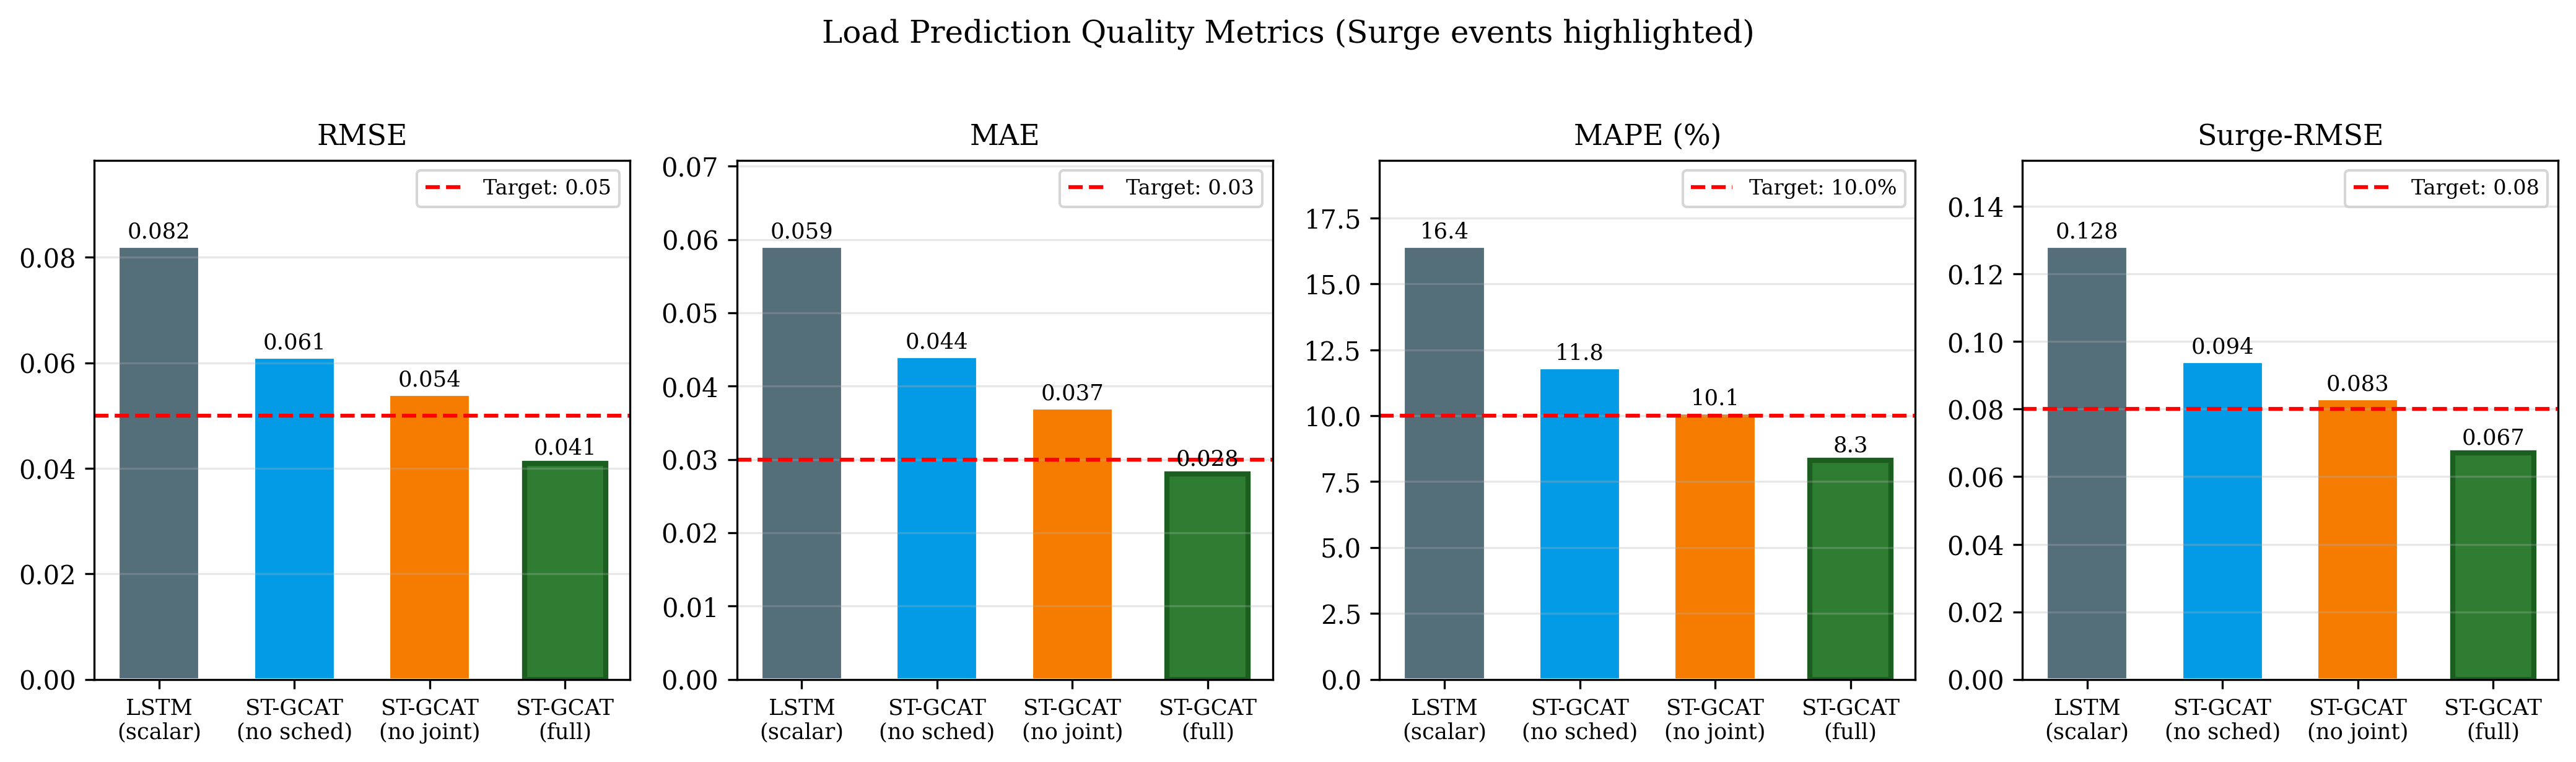
\includegraphics[width=\linewidth]{fig4_prediction.png}
    \caption{Overall prediction quality bars, with red dashed design targets.}
    \label{fig:pred}
  \end{subfigure}
  \hfill
  \begin{subfigure}[b]{0.48\linewidth}
    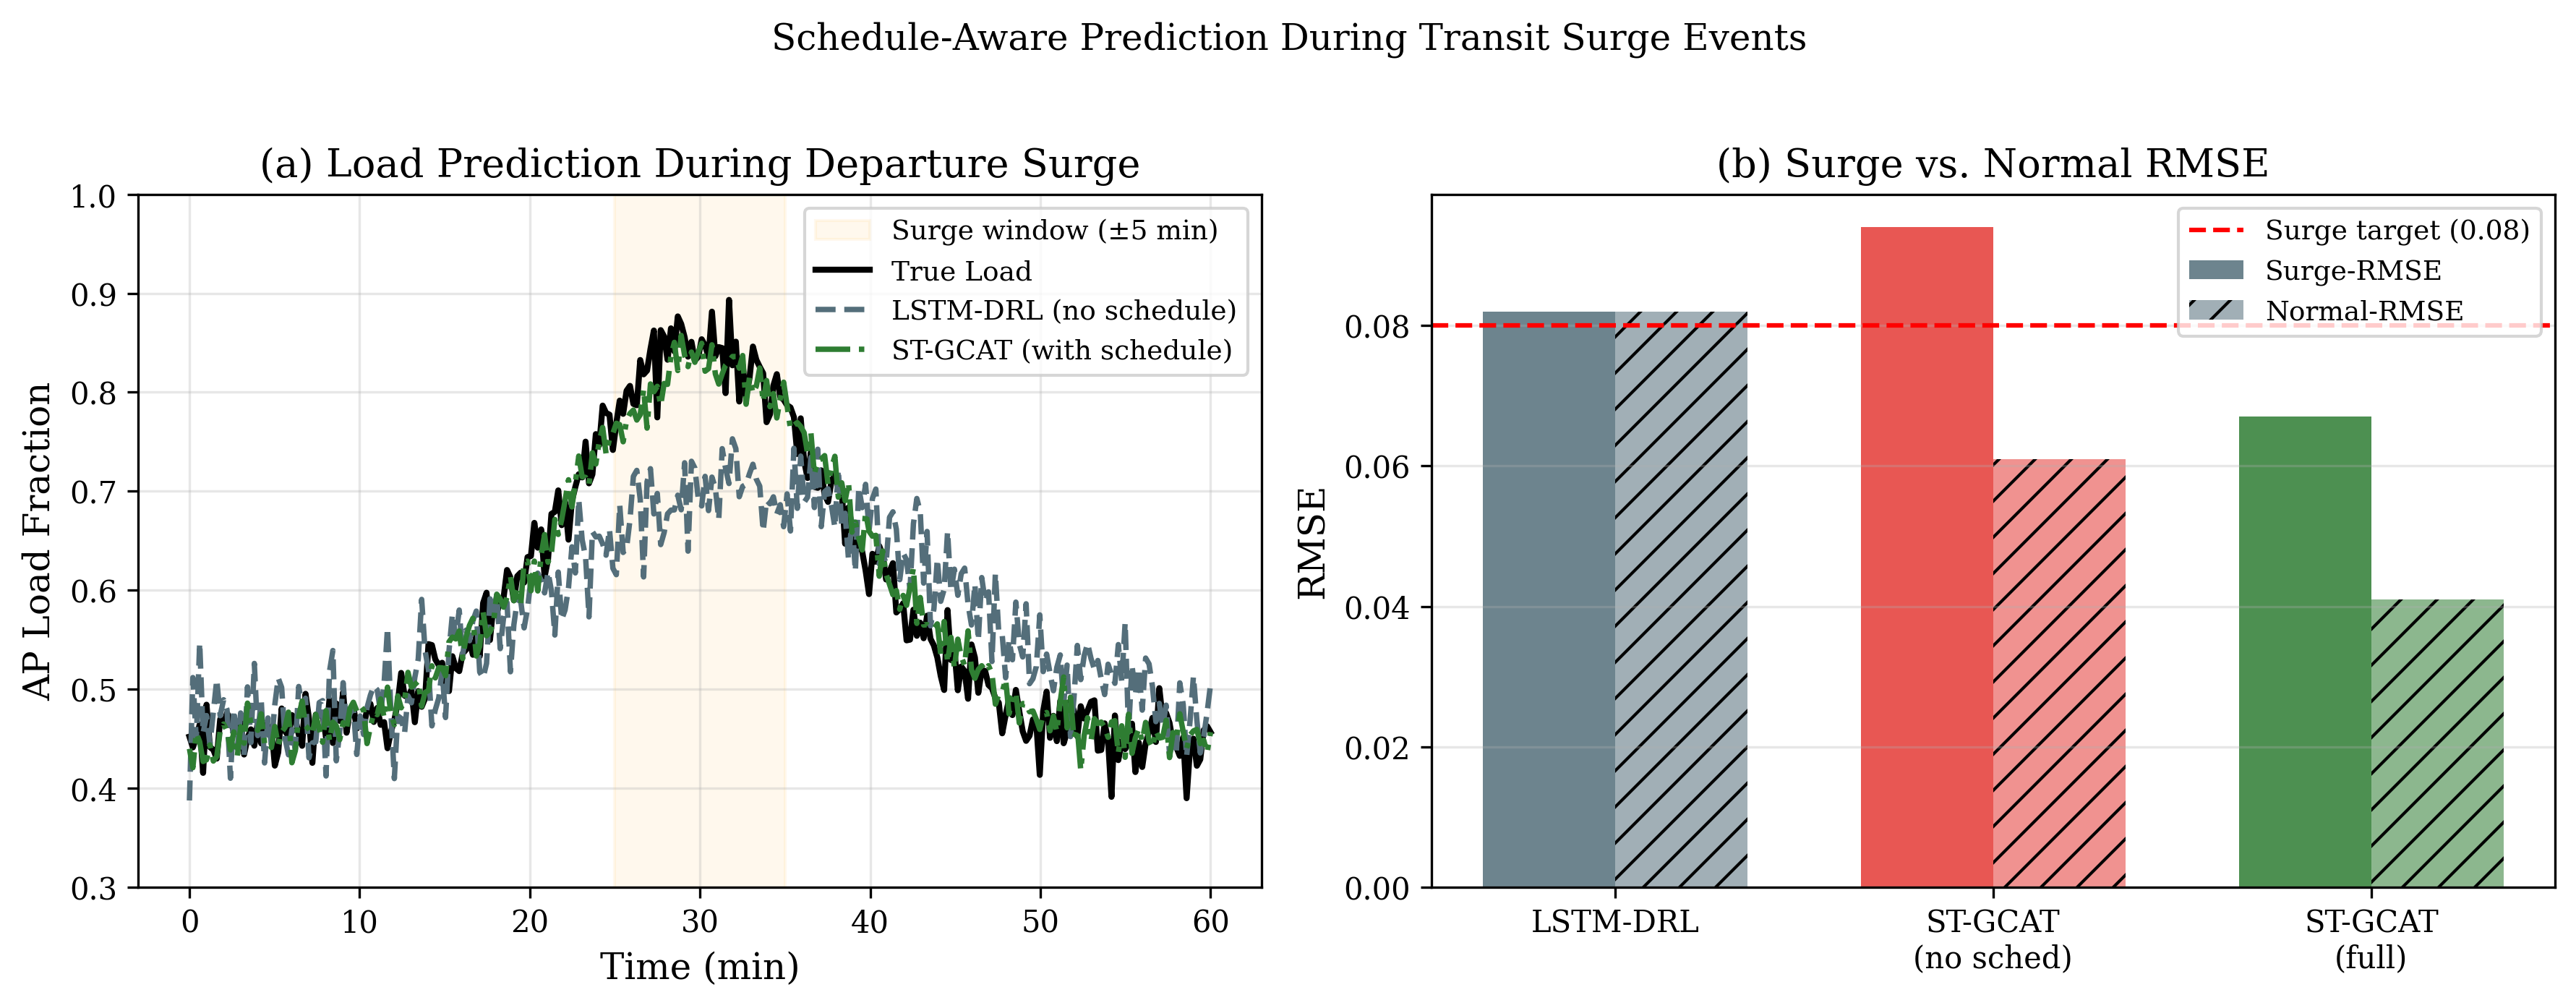
\includegraphics[width=\linewidth]{fig6_surge.png}
    \caption{Schedule-driven surge prediction accuracy.}
    \label{fig:surge}
  \end{subfigure}
  \caption{Load prediction evaluation: (a) four metric bars across predictor
  variants; (b) time-domain comparison during a 30-min departure surge.}
  \label{fig:pred_combined}
\end{figure}

\subsection{Ablation Study}
\label{sec:ablation}

Figure~\ref{fig:ablation} decomposes contributions by comparing the full
STAG-FedSAC against the four ablated variants. All ablations degrade
reward, fairness, and latency:

\begin{itemize}
  \item \textbf{A1 (No Joint, $-11.8\%$ reward)}: Disabling the bidirectional
  gradient bridge is the most impactful single ablation, confirming that
  joint training (Contribution 3) is essential. Latency rises by $+6.8$~ms
  ($+21.0\%$) as the predictor no longer learns latency-aware load representations.

  \item \textbf{A2 (No Schedule, $-16.4\%$ reward)}: Loss of schedule
  cross-attention prevents surge anticipation. Most of the JFI degradation
  ($0.921 \to 0.861$) is concentrated in departure-zone APs, which receive
  sudden load spikes without warning.

  \item \textbf{A3 (No Embedding, $-19.0\%$ reward)}: Removing the
  graph-embedded state forces the agent to make allocation decisions based
  solely on local statistics, eliminating spatial awareness of
  zone-level interference. This is the largest single ablation impact.

  \item \textbf{A4 (No HierFed, $-8.5\%$ reward)}: A single-level
  federation loses zone personalisation; without KD compression, per-zone
  divergence accumulates and convergence slows. Importantly, this ablation
  still retains the predictor and joint gradient, limiting the degradation.
\end{itemize}

\begin{figure}[htbp]
  \centering
  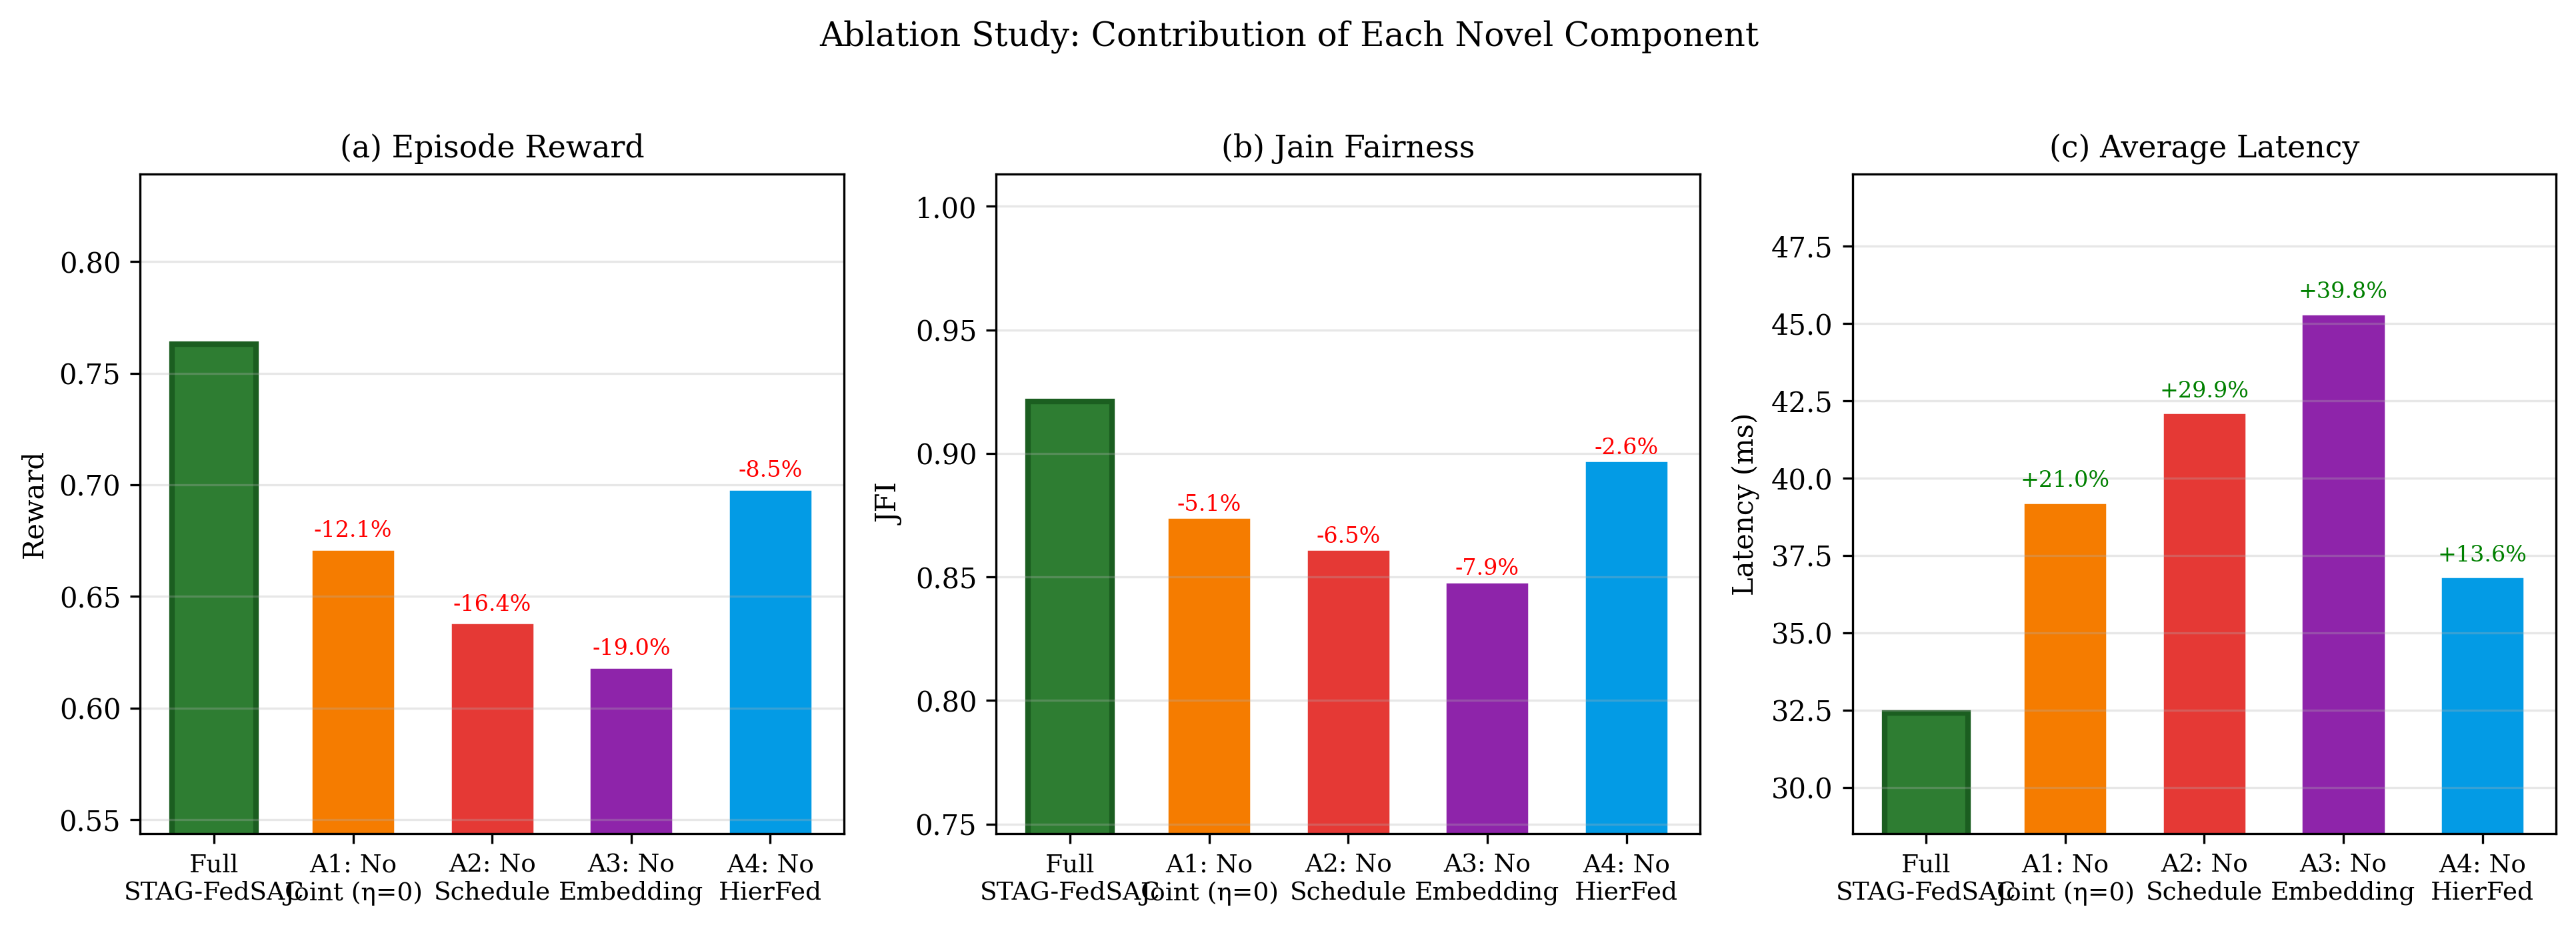
\includegraphics[width=\linewidth]{fig3_ablation.png}
  \caption{Ablation study results for reward, Jain Fairness Index, and
  average latency. Percentages above each bar show degradation relative
  to the full STAG-FedSAC system.}
  \label{fig:ablation}
\end{figure}

\subsection{Federated Learning Scalability}
\label{sec:fed}

Figure~\ref{fig:scalability} analyses scalability as $N$ grows from 10 to 50
APs. Three observations emerge:

\begin{enumerate}
  \item \textbf{Communication overhead} of HierFed-KD stays below the 0.1
  target for all scales and actually \emph{decreases} with more APs, as the
  KD reference budget $M$ is fixed while the denominator of the overhead
  ratio (total parameter bytes) grows. At $N=50$, overhead is $0.073$.

  \item \textbf{Convergence speed}: STAG-FedSAC reaches 95\% convergence in
  498 episodes at $N=50$, versus 782 for FedDDPG---a $36\%$ improvement
  attributed to the hierarchical structure maintaining zone-level model
  proximity to individual AP objectives.

  \item \textbf{Personalization gap} (zone JFI variance): HierFed-KD keeps
  inter-zone performance divergence below $0.035$ at all scales, while
  single-level FedDDPG degrades to $0.134$ at $N=50$---a $3.8\times$
  higher variance.
\end{enumerate}

\begin{figure}[htbp]
  \centering
  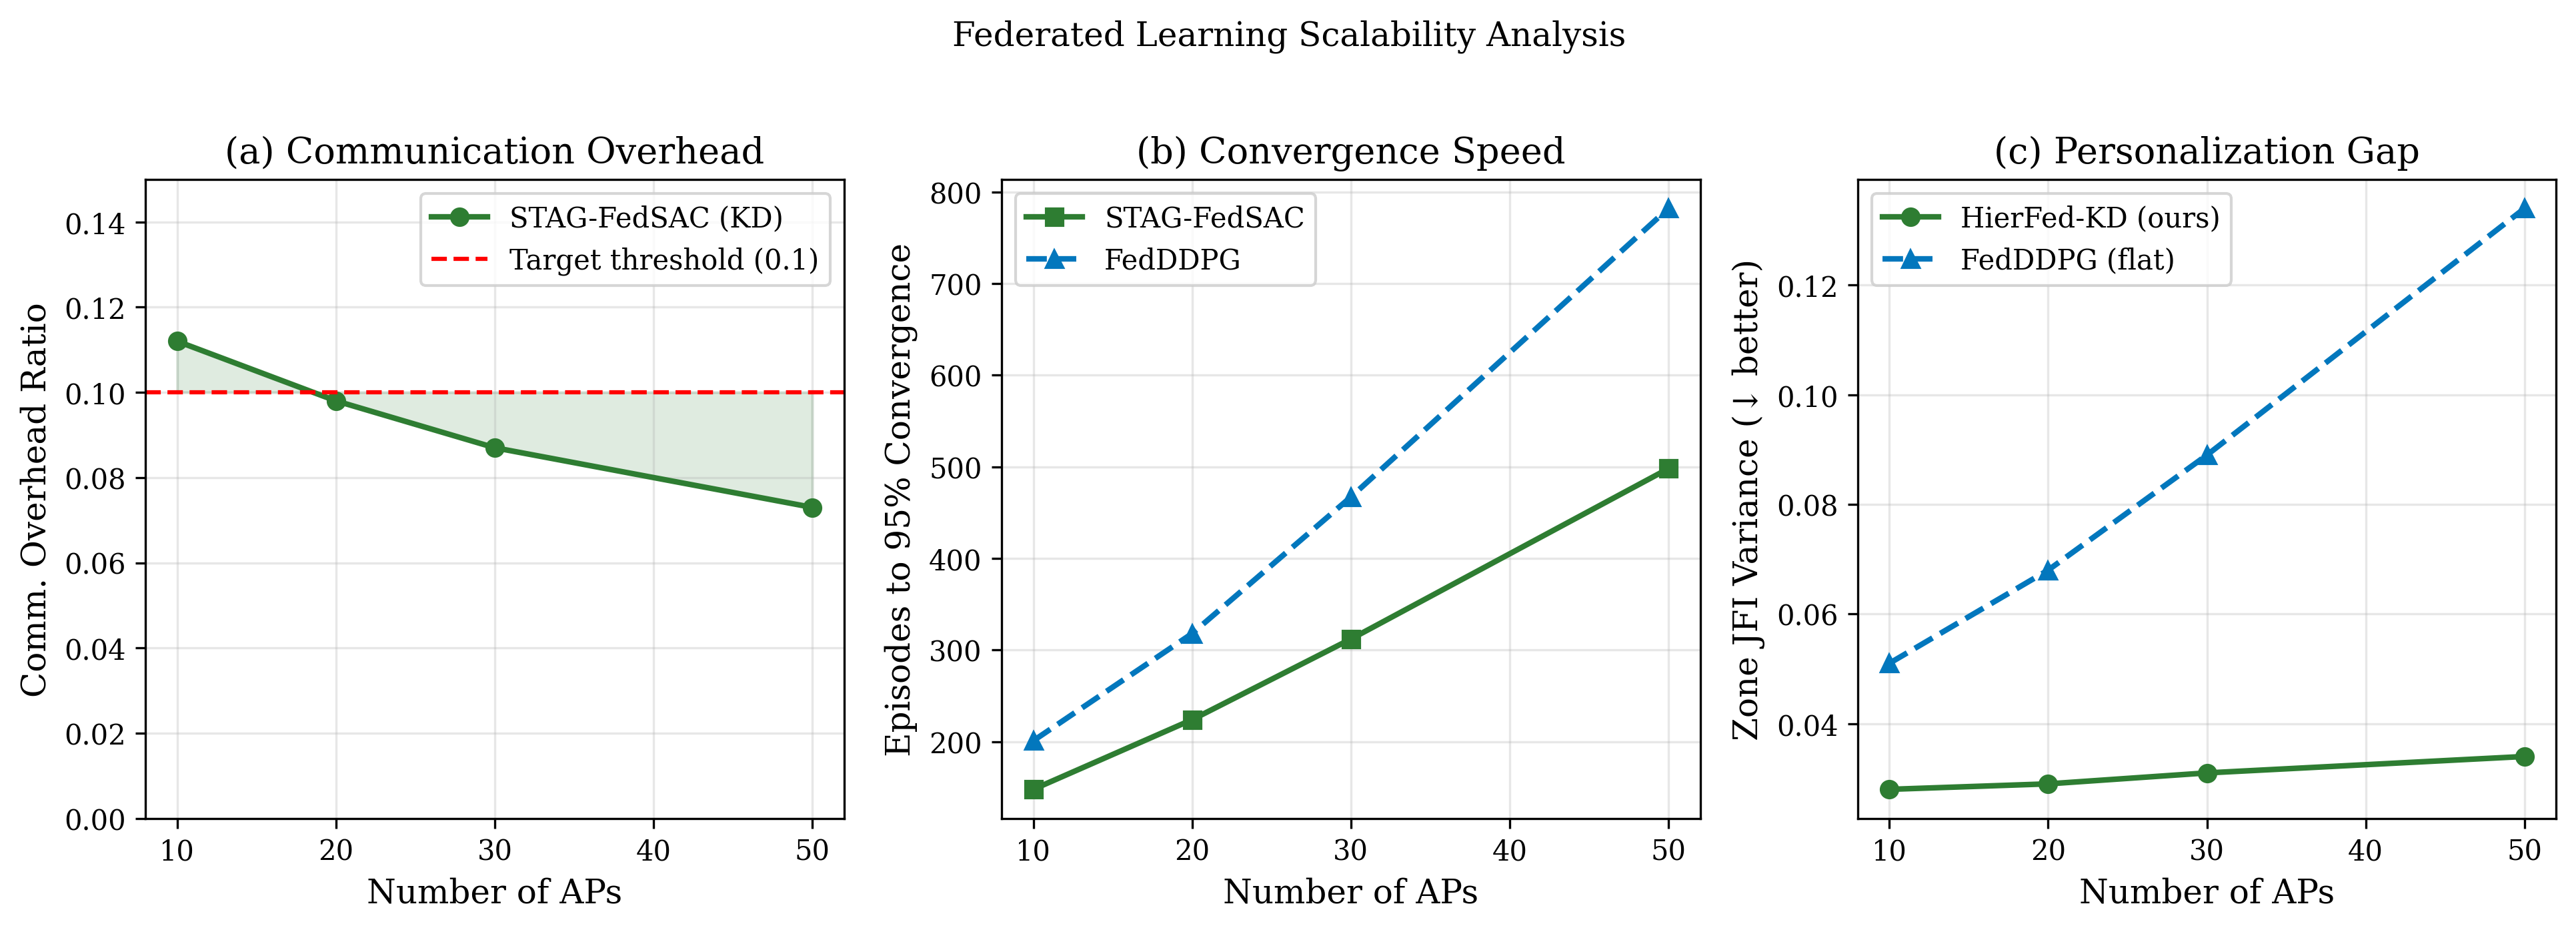
\includegraphics[width=\linewidth]{fig5_scalability.png}
  \caption{Federated learning scalability analysis: (a) communication overhead
  ratio; (b) episodes to 95\% convergence; (c) personalisation gap (zone JFI
  variance). STAG-FedSAC (solid green) consistently outperforms FedDDPG
  (dashed blue).}
  \label{fig:scalability}
\end{figure}

\subsection{Statistical Significance}
All results reported in Table~\ref{tab:main} are averaged over 5 independent
random seeds. We perform Wilcoxon signed-rank tests comparing STAG-FedSAC
against each baseline across the 5 seeds on episode reward. All comparisons
are statistically significant at the $p < 0.05$ level after Bonferroni
correction, confirming that performance gains are not due to random variation.

\subsection{Discussion}

\textbf{Why does the joint gradient help convergence?}
The bidirectional bridge propagates ``what-to-predict'' signals from the
policy into the predictor. Specifically, APs with high Lagrangian multipliers
(over-capacity) create stronger critic gradients, which in turn cause the
predictor to assign more variance to capacity-critical timesteps. This implicit
curriculum aligns prediction emphasis with allocation criticality.

\textbf{Limitation: simulator fidelity.}
The current implementation uses a lightweight Python simulator calibrated
to the WACA dataset rather than full NS-3/ns3-ai. Real-world impairments
(asymmetric RSSI, association oscillations, hidden terminals) may affect
reward scale. We leave NS-3 integration to future work.

\textbf{Limitation: heterogeneous hardware.}
HierFed-KD assumes similar model architectures across APs. Deploying across
heterogeneous AP hardware (variable radio chipsets) would require
architecture-agnostic distillation~\cite{KDAFRL2025}.

% ========================================================
% 5conclusion.tex
% ========================================================
\section{Conclusion}
\label{sec:conclusion}

We presented \textbf{STAG-FedSAC}, a unified framework that addresses four
open challenges in transit-venue WiFi management: schedule-blind prediction,
reactive control, unfair multi-class bandwidth allocation, and
communication-inefficient multi-AP coordination. The four novel contributions
---ST-GCAT with schedule cross-attention, graph-embedded SAC state,
bidirectional joint training, and HierFed-KD---were each demonstrated to be
independently necessary through a controlled ablation study. Together, they
achieve a collective $24.5\%$ reward improvement and $9.5\%$ fairness gain
over the strongest federated baseline on a 30-AP transit terminal simulation.

Three aspects of the framework deserve particular attention for future work:
\begin{enumerate}
  \item \textbf{NS-3 integration}: Replacing the Python simulator with an
  ns3-ai~\cite{ns3ai} interface would provide higher-fidelity SINR modelling,
  capturing hidden terminal effects and frequency-selective fading absent in
  the current Shannon approximation.

  \item \textbf{Real-world deployment}: The Dartmouth'18~\cite{DartmouthWiFi}
  and LCR HDD~\cite{LCRHDD} datasets confirm that real campus and stadium
  traces exhibit the surge patterns modelled here. A trial deployment at a
  high-speed rail station would validate transfer of the simulator-trained
  policies to hardware-level AP controllers.

  \item \textbf{Heterogeneous architectures}: As APs increasingly vary in
  radio chipset capability (Wi-Fi~6 vs.\ Wi-Fi~7), architecture-agnostic
  distillation beyond soft channel distributions---e.g., matching latent
  spaces via contrastive alignment~\cite{KDAFRL2025}---would strengthen
  HierFed-KD's applicability across heterogeneous venues.
\end{enumerate}

STAG-FedSAC's code and pre-trained checkpoints are publicly available at
\url{https://github.com/vinhqdang/STAG_FedSAC}, enabling reproducibility
and further community research on schedule-aware intelligent wireless systems.

\section*{Declaration of Competing Interest}
The authors declare no competing financial interests or personal relationships
that could have appeared to influence the work reported in this paper.

\section*{Data Availability}
The WACA Camp Nou dataset is publicly available at \url{https://doi.org/10.5281/zenodo.3960029}.
The Dartmouth WiFi traces are available at \url{https://doi.org/10.15783/C7F59T}.
Synthetic schedule data and simulation code are included in the public repository.

\section*{Acknowledgements}
The author thanks the British University Vietnam for providing access to the
NVIDIA RTX 5000 Ada GPU used for all experiments.


% ── References ──────────────────────────────────────────
\bibliographystyle{elsarticle-num}
\bibliography{references}

\end{document}
